\documentclass[12pt,a5paper,landscape]{scrartcl}

\usepackage{vorschule}
\usepackage[
    typ=ohne,
    fach=Mathematik,
    lerngruppe={7},
	nummer=4,
    module={Lizenzen,Symbole},
	seitenzahlen=keine,
	farbig,
    lizenz=cc-by-nc-sa-4,
]{schule}

\usepackage[
	typ=lerntheke,
	kuerzel=Ngb,
	reihe={Terme und Gleichungen},
	version={2020-12-03},
]{ngbschule}

\author{J. Neugebauer}
\title{0.1 (Terme und Gleichungen)}
\date{\Heute}

\begin{document}

\begin{hilfekarte}{Terme, Gleichungen und Variablen}{begriffe}
	Ein \textbf{Term} ist ein \emph{sinnvoller} Rechenausdruck aus Zahlen, Rechenzeichen, Vorzeichen, Klammern und Variablen.
	
	Gültig: $5+(3,4 - (-4)) + x$\\
	Ungültig: $5+\cdot5)-4$
	
	\vspace{1cm}
	Eine \textbf{Gleichung} besteht aus zwei Termen, die durch ein Gleichzeichen ($=$) verbunden sind. Eine Gleichung kann \emph{wahr} (\emph{gültig}) sein (z.B. $5+3 = 9-1$) oder \emph{falsch} sein (z.B. $4 = 1+1$).
	
	\vspace{1cm}
	Eine \textbf{Variable} ist ein Platzhalter für einen Wert, der erstmal unbekannt oder nicht festgelegt ist.
	
	\vspace{2cm} \small
	Als Kurzschreibweise für eine Multiplikation einer Zahl mit einer Variablen benutzen wir $4\cdot x = 4x$.
\end{hilfekarte}

\begin{loesungskarte}[Terme, Gleichungen und Variablen]
	Beispiele für Terme:
	\begin{multicols}{2}
		\textbf{sinnvolle Ausdrücke (Terme)}
		\begin{gather*}
		4 \\
		x \\
		4+3-5.1\cdot (7.2+5) \\
		4-a+2\cdot b \cdot c \\
		5 - \left( \frac{1}{2} - \frac{x}{3} \right)  \cdot ( 4.254 )
		\end{gather*}
		
		\textbf{unsinnige Ausdrücke (keine Terme)}
		\begin{gather*}
		+ \\
		4\cdot \\
		5+:x \\
		(4+3-(5.1\cdot (7.2+5 \\
		7..5 \$ 6 \\
		\cdot \left( \frac{\quad}{2} - \frac{x}{\quad} \right)  \cdot ( 4.254 )
		\end{gather*}
	\end{multicols}
\end{loesungskarte}


\begin{hilfekarte}{Variablen}{variablen}
	\textbf{Variablen} sind Platzhalter für Werte, die noch unbekannt sind. Wir benutzen kleine Buchstaben für Variablen (z.B: $x,y,a,b,c,\dots$). Kommt ein Buchstabe mehrfach vor, dann steht er immer für denselben Wert.
	
	Es gibt zwei Arten von Variablen:
	
	In einem \emph{Term} ist eine Variable ein Platzhalter für beliebige Werte, die du dir selber aussuchen kannst. Du kannst für die Variablen Zahlen einsetzen und den Wert des Terms berechnen. z.B.
	
	\[ 5\cdot a + 4 \overset{a = 3}{\longrightarrow} 5\cdot 3 + 4 = 19 \]
	
	In einer \emph{Gleichung} steht eine Variable für einen bestimmten Wert, der gefunden werden muss. So, dass die Gleichung wahr ist. z.B.
	
	\[ 5\cdot x + 4 = 34 \Rightarrow x = 4 \text{, da } 5\cdot 4 + 4 = 34\text{ wahr ist} \]

	Als Kurzschreibweise für eine Multiplikation einer Zahl mit einer Variablen benutzen wir $4\cdot x = 4x$.
\end{hilfekarte}

\leereKarte

\begin{hilfekarte}{Termumformungen}{termumf}
	Um Dir das Rechnen leichter zu machen können Terme durch zusammenfassen vereinfacht werden. Gültige Umformungen sind:
	
	\begin{smallitemize}
		\item Summanden ohne Variablen können zusammengefasst werden. $2 + 4 + 5$ wird zu $11$
		\item Summanden mit derselben Variablen können zusammengefasst werden. $12a - 4a + a$ wird zu $9a$
		\item Faktoren ohne Variable können mit einer Variablen multipliziert werden: $4\cdot 5\cdot 2x$ wird zu $40x$
	\end{smallitemize}
	
	Auch mit Hilfe der Rechengesetze kannst Du die Terme umformen:
	\begin{smallitemize}
		\item \emph{Kommutativgesetz}: $4a + b + 3a = 4a + 3a + b = 7a + b$
		\item \emph{Assoziativgesetz}: $5b - 2a + a = 5b + (-2a + a) = 5b - a$
		\item \emph{Distributivgesetz}: $2\cdot (a + 5) = 2\cdot a + 2\cdot 5)$
		\item \emph{Minusklammern auflösen}: $8 -(a - 5 + 3b) = 8 - a + 5 - 3b)$
	\end{smallitemize}
\end{hilfekarte}

\begin{loesungskarte}[Termumformungen]
	Beispiele:
	\begin{multicols}{2}
	\begin{align*}
		&\quad 5x + 7x - 2\cdot 3x + 2y \\
			&= 12x - 6x + 2y \\
			&= 6x + 2y
	\end{align*}

	\begin{align*}
		&\quad 6,2 \cdot (4x + 3.1y) - 5,6x \\
			&= 6,2\cdot 4x + 6,2\cdot 3,1y - 5,6x \\
			&= 24,8x + 19,22y - 5,6x \\
			&= 19,2x + 19,22y
			\end{align*}
	\end{multicols}
\end{loesungskarte}

\begin{hilfekarte}{Äquivalenzumformungen}{aequivumf}
	Führst Du auf beiden Seiten einer Gleichung dieselbe Umformung durch, dann bleibt die Gleichung weiterhin gültig.
	Rechnest Du auf der rechten Seite $-4$, musst Du also auf der anderen Seite auch $-4$ rechnen.
	\begin{alignat*}{3}
	\gl[]{4a + 5}{7a + 4} \tu[-4]\\
	\gl{4a + 5 - 4}{7a + 4 - 4} \\
	\gl{4a + 1}{7a}
	\end{alignat*}
	
	Gültige Äquivalenzumformungen sind:
	\begin{itemize}
		\item Addition/Subtraktion einer Zahl.
		\item Multiplikation mit / Division durch eine Zahl.
	\end{itemize}
\end{hilfekarte}

\begin{loesungskarte}[Äquivalenzumformungen]
	\begin{alignat*}{3}
		\gl[]{4a + 5}{7a + 4} \tu[-4]\\
		\gl{4a + 1}{7a} \tu[-4a] \\
		\gl{1}{3a} \tu[:3] \\
		\gl{\dfrac{1}{3}}{a}
	\end{alignat*}
\end{loesungskarte}

\begin{hilfekarte}{Sachaufgaben systematisch lösen}{sach}
Um eine Text- oder Sachaufgaben systematisch zu lösen, kannst Du nach diesen vier Schritten vorgehen:
\begin{enumerate}
	\item \textbf{Aufgabe verstehen}: Lies den Aufgabentext sorgfältig durch. Markiere wichtige Informationen im Text. Informiere Dich über Begriffe, die Du noch nichts kennst.
	\item \textbf{(Teil-)Probleme identifizieren}: Schreibe Dir alle wichtigen Informationen aus dem Text sorgfältig auf und notiere dir Werte und Gleichungen, die Du ablesen kannst. Am Ende stellst Du eine Gleichung auf, die Du lösen musst.
	\item \textbf{Lösung berechnen}: Löse die Gleichung mit Term- und Äquivalenzumformungen.
	\item \textbf{Probe und Rückschau}: Mache mit dem Ergebnis noch eine Proberechnung. Prüfe das Ergebnis auch im Kontext der Aufgabe: Klingt das Ergebnis realistisch? Fall nicht, musst Du noch einmal von vorne anfangen und Deinen Lösungsweg überprüfen.
\end{enumerate}

Ein Beispiel findest Du auf der Rückseite.
\end{hilfekarte}

\begin{loesungskarte}[Terme, Gleichungen und Variablen]
\begin{rahmen}
	Für \textcolor{\lsgFarbe}{zwei Erwachsene} und \textcolor{\lsgFarbe}{drei Kinder} müssen in einem Freizeitpark insgesamt \textcolor{\lsgFarbe}{\EUR{84}} gezahlt werden. \textcolor{\lsgFarbe}{Erwachsene kosten das Doppelte von Kindern.} Wie teuer ist eine Karte für ein Kind?
\end{rahmen}
	
\begin{multicols}{2}
	\textbf{Teilprobleme sammeln:} \\
	Karte Kind: $x$ \\
	Karte Erwachsener: $y$ \\
	Kosten insg.: $2\cdot y + 3\cdot x = 84$ \\
	Erwachsene kosten das Doppelte: $y = 2\cdot x$ \\
	Gleichung: $2\cdot (2\cdot x) + 3\cdot x = 84$
	
	\columnbreak
	\textbf{Gleichung lösen:}
	\begin{alignat*}{3}
		\gl[]{2\cdot (2\cdot x) + 3\cdot x}{84} \\
		\gl{4x + 3x}{84} \\
		\gl{7x}{84} \\
		\gl{x}{12}
	\end{alignat*}
\end{multicols}

\begin{hilfekarte}{Ungleichungen}
	Bei einer Ungleichung steht statt dem \emph{Gleichzeichen} ein \emph{Ungleichungszeichen} zwischen den beiden Termen. Ungleichungszeichen sind:
	\begin{itemize}
		\item[$>$] \emph{größer als}
		\item[$<$] \emph{kleiner als}
		\item[$\gt$] \emph{größer als oder gleich}
		\item[$\lt$] \emph{kleiner als oder gleich}
	\end{itemize}
	
	Wie eine Gleichung kann eine Ungleichung wahr oder falsch (Gültig oder ungültig) sein:
	\begin{itemize}
		\item Gültig: $4 < 5$
		\item Ungültig: $4 \gt 5$
	\end{itemize}
	
	Ungleichungen mit einer Variablen können (fast) wie Gleichungen umgeformt werden. Die Lösung sind aber meist mehrere Zahlen:
	\begin{itemize}
		\item $x < 5$ Lösung: Alle Zahlen die kleiner als $5$ sind (aber nicht die $5$ selber).
		\item $x \gt 4.3$ Lösung: Alle Zahlen die größer oder gleich $4.3$ sind (also auch $4.3$ selber).
	\end{itemize}
\end{hilfekarte}

\textbf{Probe und Rückschau:} \\
$4\cdot 12 + 3\cdot 12 = 48 + 36 = 84$ \checkmark\\[5mm]
Das Ergebnis scheint realistisch. (Der Potts Park in Minden kostet zum Beispiel \EUR{23,50} für einen Erwachsenen.)
\end{loesungskarte}

\begin{karte1}{Terme vereinfachen}
\hilfeMarke{termumf}
	Löse die Klammern auf und vereinfache die Terme.
	
	\begin{tasks}(2)
		\task $28 + (15x + 12) \cdot 3$
		\task $15a - (2a + 3) - (-x)$
		\task $9 - 2\cdot ( k-3) - 3$
		\task $-(h + 1) + 25 -3h$
		\task $9 \cdot(2y + 3)$
		\task $7-(4-5\cdot x)$
	\end{tasks}
\end{karte1}

\begin{loesungskarte}
	\begin{tasks}(2)
		\task $64 + 45x$
		\task $14x - 3$
		\task $-2k$
		\task $-4h + 24$
		\task $18y + 27$
		\task $3 + 5x$
	\end{tasks}
\end{loesungskarte}

\begin{karte1}{Gleichungen lösen}
\hilfeMarke{aequivumf}
	Löse die Gleichungen mit Hilfe von Äquivalenzumformungen.
	
	\begin{tasks}(2)
		\task $32 - 4\cdot (2x - 5) = 59 -x $
		\task $4z - 15 = 45 - 2z$
		\task $0,9a + 2,5 = 2,4a - 2$
		\task $\dfrac{4}{5} \cdot \left( \dfrac{3}{4} \cdot x + 3 \right) = 4 - \dfrac{2}{5}\cdot  x$
		\task $-\dfrac{2}{3}x - \dfrac{8}{18} = -\dfrac{1}{9}x - 1$
		\task $\dfrac{7}{6} - 6x = -2 + \dfrac{8}{5}x$
	\end{tasks}
\end{karte1}

\begin{loesungskarte}
	\begin{tasks}(2)
		\task $x = -1$
		\task $z = 10$
		\task $a = \dfrac{1}{3}$
		\task $x = \dfrac{8}{5} = 1,6$
		\task $x = 1$
		\task $x = -\dfrac{25}{228}$
	\end{tasks}
\end{loesungskarte}

\begin{karte1}{Zahlenrätsel}
\hilfeMarke{aequivumf}
	\begin{wrapfigure}[12]{r}{0pt}
		
\includegraphics[width=4cm]{7.4-LT-Abb_Nachdenken}
	\end{wrapfigure}
	
	Löse das Zahlenrätsel, indem Du eine Gleichung aufstellst.
	
	\begin{enumeratea}
		\item Wird $8$ vom Dreifachen einer Zahl subtrahiert, erhält man 7.
		\item Addiert man zum Fünffachen einer Zahl 9, so erhält man die Differenz aus 21 und der Zahl.
		\item Addieret man zur Hälfte einer Zahl 4, vervierfache das Ergebnis und subtrahiere die Zahl, so erhält man 4.
		\item Das Produkt aus einer Zahl und 7 ist genauso groß wie die Differenz von 32 und der Zahl.
		\item Die Summe dreier aufeinander folgender Fünferzahlen ist 135.
	\end{enumeratea}
\end{karte1}

\begin{loesungskarte}
	\begin{enumeratea}
		\item $3x - 8 = 7$ \hspace{1cm} Die Zahl ist $5$.
		\item $5x + 9 = 21 - x$ \hspace{1cm} Die Zahl ist $2$.
		\item $4\cdot (0,5x + 4) - x = 4$ \hspace{1cm} Die Zahl ist $-12$.
		\item $z\cdot  7 = 32 - z$  \hspace{1cm} Die Zahl ist $4$.
		\item $z + (z+5) + (z+10) = 135$ \hspace{1cm} Die Zahlen sind $40$, $45$ und $50$.
	\end{enumeratea}
\end{loesungskarte}

\begin{karte2}{Finde den Fehler}
\hilfeMarke{aequivumf}
	Was wurde hier jeweils falsch gemacht? Erkläre den Fehler und berichtige ihn dann.
	
	\begin{tasks}(2)
		\task 
		\begin{alignat*}{3}
			\gl[]{3x+1}{4x-2} \\
			\gl{1}{x-2} \\
			\gl{-1}{x}
		\end{alignat*}
		
		\task 
		\begin{alignat*}{3}
			\gl[]{\dfrac{1}{2}x+2}{5} \\
			\gl{\dfrac{1}{2}x}{3} \\
			\gl{x}{\dfrac{3}{2}}
		\end{alignat*}
		
		\task 
		\begin{alignat*}{3}
			\gl[]{0,75x+4}{1,25x} \\
			\gl{4}{2x} \\
			\gl{2}{x}
		\end{alignat*}
		
		\task
		\begin{alignat*}{3}
			\gl[]{3\cdot (2-x)}{2x-(x+6)} \\
			\gl{6-3x}{x+6} \\
			\gl{6}{2x} \\
			\gl{x}{3}
		\end{alignat*}
	\end{tasks}
\end{karte2}

\begin{loesungskarte}
	\begin{tasks}(2)
		\task Im letzten Schritt wurde auf der linken Seite $-2$ statt $+2$ gerechnet.
		\task Im letzten Schritt wurde auf der rechten Seite $\cdot\dfrac{1}{2}$ gerechnet und nicht $:\dfrac{1}{2}$ bzw. $\cdot 2$.
		\task Im ersten Schritt wurde auf der rechten Seite $+0,75x$ gerechnet und nicht $-0,75x$.
		\task Im zweiten Schritt muss die Gleichung $6-6=x+3x$ gerechnet werden. Zusammengefasst muss die dritte Gleichung also $0=4x$ lauten.
	\end{tasks}
\end{loesungskarte}

\begin{karte1}{Sachaufgaben}
\hilfeMarke{sach}
	\begin{enumeratea}
		\item Christine ist 4 Jahre älter als Martin. Martin ist 3 Jahre jünger als Sebastian. Zusammen sind sie 109 Jahre alt. Wie alt ist jeder?
		\item Der Suezkanal ist ein großes Bauwerk der Menschheit. Im Jahr 2019 ist er dreimal so alt, wie er im Jahr 1919 war. Bestimme, wann der Suezkanal eröffnet wurde.
	\end{enumeratea}
	
	\begin{center}
		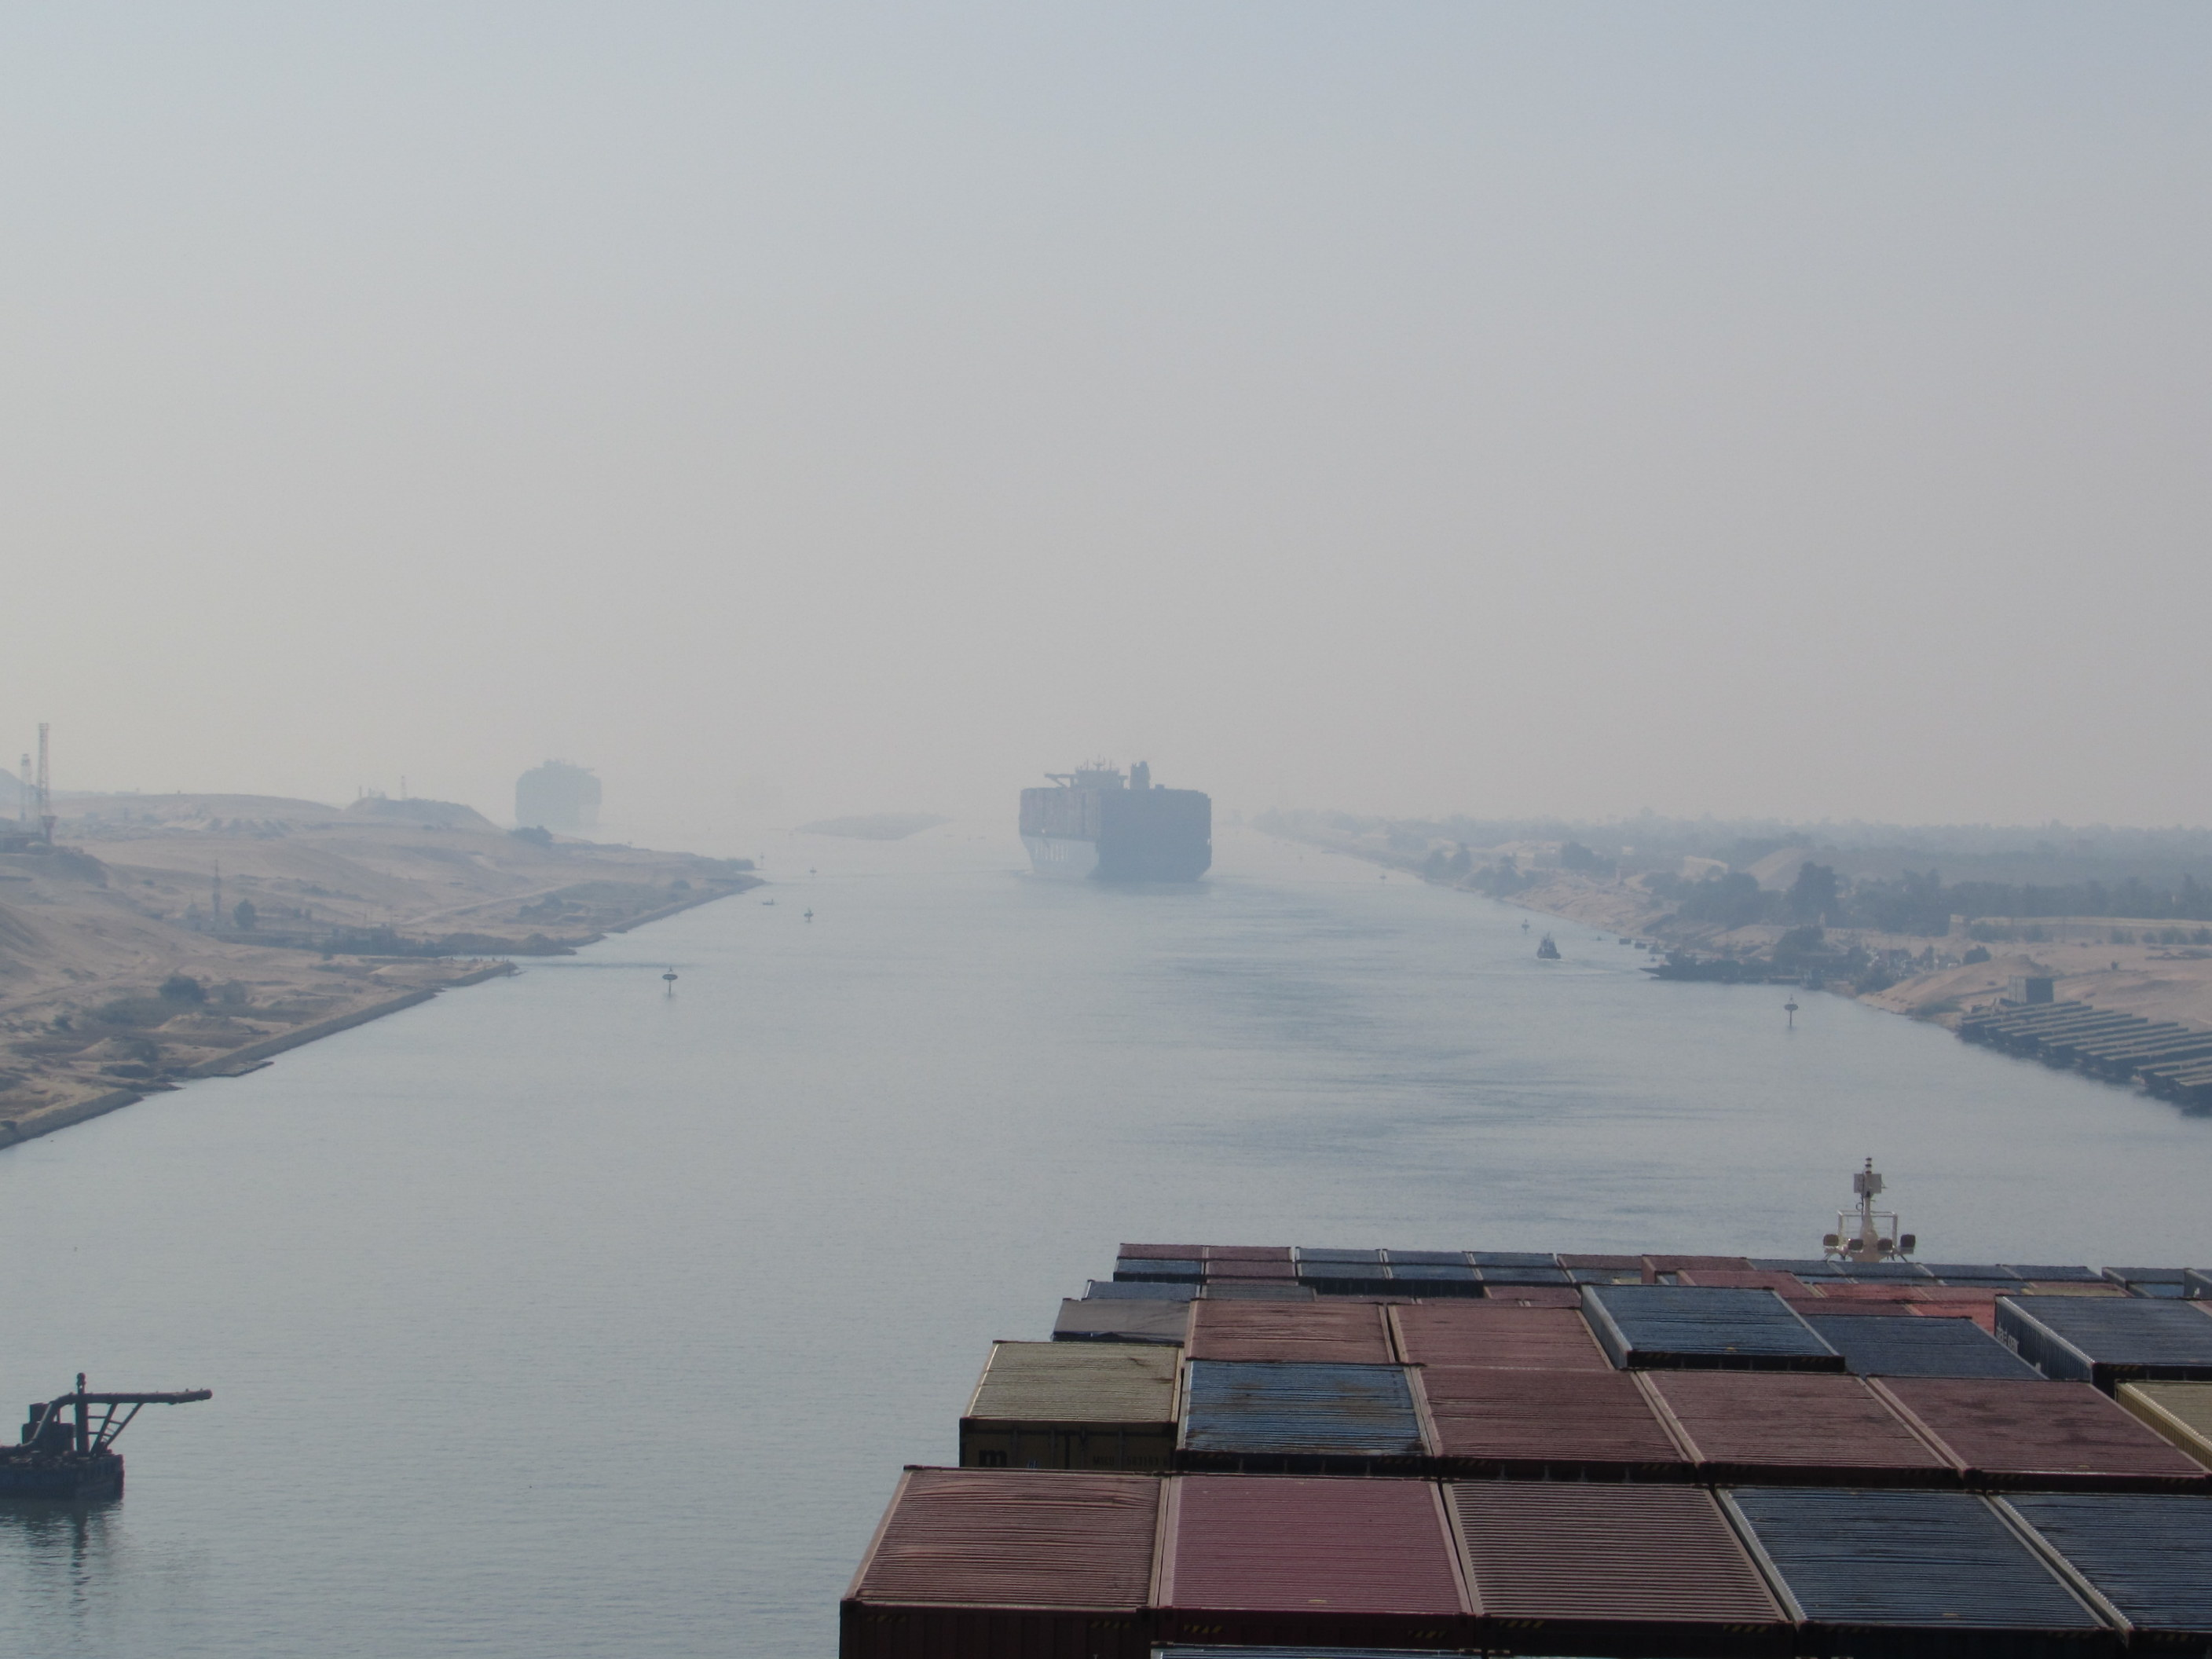
\includegraphics[width=6cm]{7.4-LT-Abb_Suezkanal_by_pass}
	\end{center}
	
	\infotext{Bildquelle: Gregor Rom unter cc-by-sa-4.0}
\end{karte1}

\begin{loesungskarte}
	\begin{enumeratea}
		\item 
		\begin{smallitemize}
			\item Martin: $m$
			\item Christine: $m+4$
			\item Sebastian: $m+3$
			\item Zusammen: $(m+4) + (m+3) + m = 109$
		\end{smallitemize}
		
		Antwort: Martin ist 34 Jahre, Christine 38 Jahre und Sebastian 37 Jahre alt.
		
		\item
		\begin{smallitemize}
			\item Alter 1919: $a$
			\item Jahr der Eröffnung: $1919-a$
			\item Alter 2019: $a+100$
			\item 2019 ist er dreimal so alt wie 1919: $3\cdot a = a+100$
		\end{smallitemize}
		
		Antwort: Der Suezkanal wurde im Jahr 1869 eröffnet.
	\end{enumeratea}
\end{loesungskarte}

\begin{karte2}{Sachaufgaben II}
\hilfeMarke{sach}
	\begin{enumeratea}
		\item Frau Fauna hat auf ihrem Balkon zwei Sorten von Tomaten gepflanzt. Die gewöhnliche Tomatenpflanze ist jetzt \SI{48}{\centi\meter} hoch und wächst \SI{6}{\centi\meter} pro Woche. Die \enquote{Cherry}-Tomate ist am selben Tag \SI{24}{\centi\meter} hoch und wächst \SI{8}{\centi\meter} pro Woche. In wie vielen Wochen haben die Pflanzen die gleiche Höhe?
		\item Die Klasse 7c hat eine Umfrage zum Schulweg gemacht: Die Hälfte der Klasse kommt mit Bus und Bahn, ein Drittel mit dem Fahrrad und die restlichen fünf kommen zu Fuß. Wie viele Kinder sind in der Klasse?
	\end{enumeratea}
\end{karte2}

\begin{loesungskarte}
	\begin{enumeratea}
		\item 
		\begin{smallitemize}
			\item Zeit in Wochen: $w$
			\item gewöhnliche Tomate in $w$ Wochen: $\SI{48}{\centi\meter} + w\cdot \SI{6}{\centi\meter}$
			\item \enquote{Cherry}-Tomate in $w$ Wochen: $\SI{24}{\centi\meter} + w\cdot \SI{8}{\centi\meter}$
			\item Zusammen: $48 + 6w = 24 + 8w$
		\end{smallitemize}
		
		Antwort: In 12 Wochen haben die beiden Pflanzen die gleich Höhe.
		
		\item
		\begin{smallitemize}
			\item Anzahl Kinder in der 7c: $k$
			\item zu Fuß: $5$
			\item mit dem Rad: $\dfrac{k}{3}$
			\item mit Bus und Bahn: $\dfrac{k}{2}$
			\item Zusammen: $k = 5 + \dfrac{k}{3} + \dfrac{k}{2}$
		\end{smallitemize}
		
		Antwort: In der Klasse 7c sind 30 Kinder.
	\end{enumeratea}
\end{loesungskarte}

\begin{karte2}{Ungleichungen}
\hilfeMarke{aequivumf}
	Finde durch Äquivalenzumformungen heraus, welche Zahlen man für $x$ einsetzen kann. Führe anschließend auch eine Probe durch.
	
	\begin{tasks}(2)
		\task $2x + 5 < 7$
		\task $5x - 5 > 35$
		\task $7 + 6x \leq 49$
		\task $2x - 3 \geq x + 1$
		\task $2x - 5 > 2$
		\task $7x - 3 \leq 3(x-1) + 5$
	\end{tasks}
\end{karte2}

\begin{loesungskarte}
	\begin{tasks}(2)
		\task $x < 1$
		\task $x > 8$
		\task $x \leq 7$
		\task $x \geq 4$
		\task $x > 3,5$
		\task $x \leq \dfrac{5}{4}$
	\end{tasks}
\end{loesungskarte}

\begin{karte1}[\symHandy]{Begreifbare Gleichungen}
\hilfeMarke{aequivumf}
\vspace*{2cm}
\begin{wrapfig}
	\begin{wrapfigure}[6]{l}{4cm}
	
\includegraphics[width=4cm]{7.4-LT-Abb_Algebra Touch}
	\end{wrapfigure}
	Hol dir ein \emph{iPad} und starte die App \programm{Algebra Touch}. Wähle rechts die Lektion \enquote{Gleichungen} und bearbeite die 16 Aufgaben für \enquote{Anfänger} und \enquote{Könner}.

	
	Du kannst jederzeit oben rechts Hilfe bekommen.
\end{wrapfig}
\end{karte1}

\leereKarte

\begin{karte2}[\symHandy]{Begreifbare Gleichungen II}
\hilfeMarke{aequivumf}
\vspace*{2cm}
\begin{wrapfig}
	\begin{wrapfigure}[6]{l}{0pt}
	
\includegraphics[width=4cm]{7.4-LT-Abb_Maphi}
	\end{wrapfigure}
	Hol dir ein \emph{iPad} und starte die App \programm{Maphi}. Wähle \enquote{Alle Kapitel} und suche die Kategorie \enquote{Lineare Gleichungen}. Scroll nach unten zum Abschnitt \enquote{Üben} und bearbeite jeweils 10 Aufgaben unter \enquote{Grundlagen} und \enquote{Weiterführend}. 
	
	Auf dem Schlüssel-Symbol unten in der Mitte kannst Du Hilfe bekommen.
\end{wrapfig}
\end{karte2}

\leereKarte

\begin{karte2}[\symHandy]{Gleichungen lösen}
\hilfeMarke{aequivumf}
\vspace*{2cm}
\begin{wrapfig}
	\begin{wrapfigure}[10]{l}{0pt}
	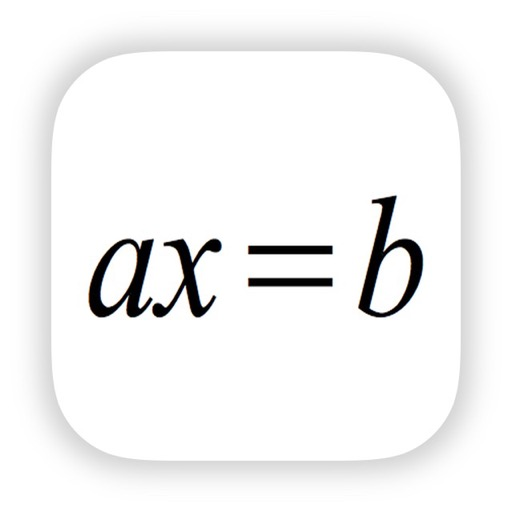
\includegraphics[width=4cm]{7.4-LT-Abb_Lineare Gleichungen}
	\end{wrapfigure}
	Hol dir ein \emph{iPad} und starte die App \programm{Gleichungen}. Wähle \enquote{Lineare Gleichungen} und suche dir einen Level aus. Löse mindestens sechs Aufgaben. 
	
	Wenn Du nicht weiter kommst, dann kannst Du dir die Komplettlösung anzeigen lassen. Dann gilt die Aufgabe aber nicht als gelöst. Verstehst Du die Aufgabe nicht, kannst Du dir eine Neue Aufgabe generieren lassen.
\end{wrapfig}
\end{karte2}

\leereKarte

\begin{karte3}{Weinkeller}
\hilfeMarke{sach}
	\begin{wrapfigure}[12]{r}{0pt}
	
\includegraphics[width=4cm]{7.4-LT-Abb_Wein}
	\end{wrapfigure}

	Ein Sommelier hat in seinem Weinkeller 200 Flaschen Wein. Ein Prozent davon ist Weißwein, der Rest ist Rotwein.\\[1em]
	
	Wie viele Flaschen Rotwein muss der Sommelier trinken, damit der Anteil an Weißwein auf zwei Prozent steigt?
	
	\infotext{Bildquelle: openclipart.org - Autor: johnny\_automatic}
\end{karte3}

\begin{loesungskarte}
	\begin{multicols}{2}\small
		Flaschen insgesamt: $200$ \\
		Flaschen Weißwein: $1\%\text{ von }200 = 200\cdot 0,01 = 2$ \\
		Flaschen Rotwein: $200-2 = 198$
		
		Anzahl Rotweinflaschen zu trinken: $x$ \\
		Neue Anzahl Weinflaschen: $200-x$ \\
		Zwei Prozent von der neuen Anzahl: $(200-x)\cdot 0,02$
	\end{multicols}

	Gleichung: $(200-x)\cdot 0,02 = 2$
	\begin{alignat*}{3}
		\gl[]{(200-x)\cdot 0,02}{2} \tu(vereinfachen) \\
		\gl{4 - 0,02x}{2} \tu[-4] \\
		\gl{-0,02x}{-2} \tu[:(-0,02)] \\
		\gl{x}{100}
	\end{alignat*}
	
	Probe: $(200-100)\cdot 0,02 = 100\cdot 0,02 = 2$
\end{loesungskarte}

\end{document}
